\begin{problem}[1]
  Use polar coordinates to evaluate the following integrals.
  \begin{enumerate}
    \item $\displaystyle\int_0^1 \int_x^{\sqrt{2-x^2}} \frac{y^2}{x^2 + y^2}
      \,\dy \,\dx$.

    \item $\displaystyle\int_0^4 \int_0^{\sqrt{4x-x^2}} \sqrt{x^2 + y^2} \,\dy
      \,\dx$.
  \end{enumerate}
\end{problem}

\begin{proof}[Solution to (i)]
  Graphing the bounds gives us
    \begin{center}
    \begin{tikzpicture}
      \begin{axis}[
          xmin=-2.5, xmax=2.5,
          ymin=-2.5, ymax=2.5,
        ]
        \addplot[samples=1000, domain=-sqrt(2):sqrt(2)+2] {sqrt(2-x^2)};
        \addplot[] {x};
        \addplot[asymptote] ({1}, x);
        \addplot[asymptote] ({0}, x);
      \end{axis}
    \end{tikzpicture}
  \end{center}

  From this, we can tell what our $\theta$ bounds are $\sfrac{\pi}{4} \le \theta
  \le \sfrac{\pi}{2}$. The bounds for $r$ are $0 \le r \le \sqrt{2}$. Converting
  the function $f(x, y) = \frac{y^2}{x^2 + y^2}$ to polar gives us $f(r, \theta)
  = \frac{r^2\sin^2(\theta)}{r^2} = \sin^2(\theta)$. Expanding and evaluating
  the double integral gives us
  \begin{align*}
    V = \iint_D \frac{y^2}{x^2 + y^2} \,\dA &= \int_{\sfrac{\pi}{4}}^{\sfrac{\pi}{2}} \int_0^{\sqrt{2}} \sin^2(\theta) \cdot r \,\dr \,\dd{\theta} \\
                                            &= \int_{\sfrac{\pi}{4}}^{\sfrac{\pi}{2}} \int_0^{\sqrt{2}} \sin^2(\theta) \cdot r \,\dr \,\dd{\theta} \\
                                            &= \int_{\sfrac{\pi}{4}}^{\sfrac{\pi}{2}} \left. \frac{r^2\sin^2(\theta)}{2} \right\rvert_0^{\sqrt{2}} \,\dd{\theta} \\
                                            &= \int_{\sfrac{\pi}{4}}^{\sfrac{\pi}{2}} \frac{2\sin^2(\theta)}{2} \,\dd{\theta} \\
                                            &= \int_{\sfrac{\pi}{4}}^{\sfrac{\pi}{2}} \frac{1 - \cos(2\theta)}{2} \,\dd{\theta} \\
                                            &= \left. \frac{\theta}{2} - \frac{\sin(2\theta)}{4} \right\rvert_{\sfrac{\pi}{4}}^{\sfrac{\pi}{2}} \\
                                            &= \left[\frac{\sfrac{\pi}{2}}{2} - \frac{\sin\left(2 - \sfrac{\pi}{4}\right)}{4}\right] - \left[\frac{\sfrac{\pi}{4}}{2} - \frac{\sin\left(2 - \sfrac{\pi}{4}\right)}{4}\right] \\
                                            &= \frac{\pi}{4} - \frac{\pi}{8} + \frac{1}{4} \\
                                            &= \frac{\pi}{8} + \frac{1}{4}
  .\qedhere\end{align*}
\end{proof}

\begin{proof}[Solution to (ii)]
  Graphing the bounds gives us
    \begin{center}
    \begin{tikzpicture}
      \begin{axis}[
          xmin=-1, xmax=5,
          ymin=-1, ymax=3,
          xtick={1, 2, 3, 4}, ytick={1, 2},
        ]
        \addplot[samples=1000, domain=0:4] {sqrt(4*x-x^2)};
        \addplot[asymptote] {0};
        \addplot[asymptote] ({4}, x);
        \addplot[asymptote] ({0}, x);
      \end{axis}
    \end{tikzpicture}
  \end{center}

  Clearly, from the graph, we see the bounds of $\theta$ to be $0 \le \theta \le
  \sfrac{\pi}{2}$. Converting the function $y = \sqrt{4x - x^2}$ to polar gives
  us
  \begin{align*}
    y^2 &= 4x - x^2 \implies 4 = (x - 2)^2 + y^2 \\
    4 &= (r\cos(\theta) - 2)^2 + r^2\sin^2(\theta) \\
    4 &= r^2\cos^2(\theta) - 4r\cos(\theta) + 4 + r^2\sin^2(\theta) \\
    r^2 &= 4r\cos(\theta) \\
    r &= 4\cos(\theta)
  .\end{align*}
  This gives us the bounds for $r$ as $0 \le r \le 4\cos(\theta)$. Converting
  the function $f(x, y) = \sqrt{x^2 + y^2}$ to polar gives us $f(r, \theta) =
  \sqrt{r^2} = r$. Expanding and evaluating the double integral gives us
  \begin{align*}
    V = \iint_D f(x, y) \,\dA &= \int_0^{\sfrac{\pi}{2}} \int_0^{4\cos(\theta)} r \cdot r \,\dr \,\dx \\
                              &= \int_0^{\sfrac{\pi}{2}} \left. \frac{r^3}{3} \right\rvert_0^{4\cos(\theta)} \,\dd{\theta} \\
                              &= \int_0^{\sfrac{\pi}{2}} \frac{64\cos^3(\theta)}{3} \,\dd{\theta} \\
                              &= \frac{1}{3} \cdot \int_0^{\sfrac{\pi}{2}} 64\cos^2(\theta)\cos(\theta) \,\dd{\theta} \\
                              &= \frac{1}{3} \cdot \int_0^{\sfrac{\pi}{2}} 64(1 - \sin^2(\theta))\cos(\theta) \,\dd{\theta}
  .\end{align*}
  Using $u$-sub, let $u = \sin(\theta)$, which gives us $\du = \cos(\theta)
  \,\dd{\theta}$. Changing the bounds gives us $u(0) = 0$ and $u(\sfrac{\pi}{2})
  = 1$. Then, we get
  \begin{align*}
    \frac{1}{3} \cdot \int_0^{\sfrac{\pi}{2}} 64(1 - \sin^2(\theta))\cos(\theta) \,\dd{\theta} &= \frac{1}{3} \cdot \int_0^1 64(1 - u^2) \,\du \\
                                                                                               &= \frac{1}{3} \cdot \int_0^1 64 - 64u^2 \,\du \\
                                                                                               &= \frac{1}{3} \cdot \left[64u - \frac{64u^3}{3}\right]_0^1 = \frac{1}{3} \cdot \left(64 - \frac{64}{3}\right) = \frac{128}{9}
  .\qedhere\end{align*}
\end{proof}

\begin{problem}[2]
  Use polar coordinates to rewrite the sum as a single iterated integral and
  then evaluate the integral.
  \[%
    \int_{\sfrac{1}{\sqrt{2}}}^1 \int_{\sqrt{1-x^2}}^x \frac{1}{x^2 + y^2} \,\dy \,\dx + \int_1^{\sfrac{3}{\sqrt{2}}} \int_0^x \frac{1}{x^2 + y^2} \,\dy \,\dx + \int_{\sfrac{3}{\sqrt{2}}}^3 \int_0^{\sqrt{9-x^2}} \frac{1}{x^2 + y^2} \,\dy \,\dx
  .\]%
\end{problem}

\begin{proof}[Solution]
  Graphing the bounds and removing all the redundant integrals gives us
  \begin{center}
    \begin{tikzpicture}
      \begin{axis}[
          xmin=-1, xmax=5,
          ymin=-1, ymax=3,
          xtick={1, 2, 3, 4}, ytick={1, 2},
        ]
        \addplot[samples=1000, domain=1/sqrt(2):1] {sqrt(1-x^2)};
        \addplot[samples=1000, domain=3/sqrt(2):3] {sqrt(9-x^2)};
        \addplot[domain=1/sqrt(2):3/sqrt(2)] {x};
        \addplot[domain=1:3] {0};
      \end{axis}
    \end{tikzpicture}
  \end{center}

  Notice that this is just the area between the two circles $x^2 + y^2 = 1$ and
  $x^2 + y^2 = 9$. Since the left hand side is stopped by the line $y = x$, we
  get the angle to be from $0$ to $\sfrac{\pi}{4}$. Converting the function
  $f(x, y) = \frac{1}{x^2 + y^2}$ to polar gives us $f(r, \theta) =
  \frac{1}{r^2}$. Expanding and evaluating the double integral gives us
  \[%
    V = \iint_D f(x, y) \,\dA = \int_0^{\sfrac{\pi}{4}} \int_1^3 \frac{1}{r^2} \cdot r \,\dr \,\dd{\theta} = \int_0^{\sfrac{\pi}{4}} \,\dd{\theta} \cdot \int_1^3 \frac{1}{r} \,\dr = \frac{\pi}{4} \cdot \left(\ln(r)\right)_1^3 = \frac{\pi\ln(3)}{4}
  .\qedhere\]%
\end{proof}

\begin{problem}[3]
  Use a double integral to find the volume of the following solids.
  \begin{enumerate}
    \item The solid that is inside the sphere $x^2 + y^2 + z^2 = 9$ and outside
      the circular cylinder $x^2 + y^2 = 4$.

    \item The solid that is bounded by the elliptic paraboloids $z = x^2 + 3y^2$
      and $z = 16 - 3x^2 - y^2$.
  \end{enumerate}
\end{problem}

\begin{proof}[Solution to (i)]
  Graphing the bounds gives us
  \begin{center}
    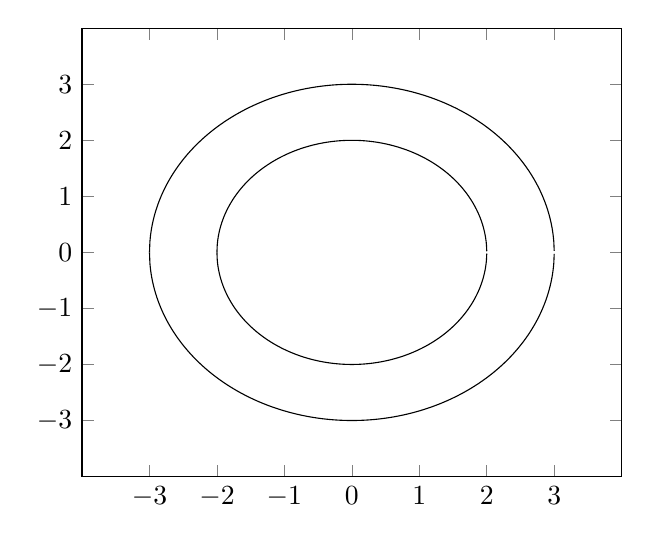
\begin{tikzpicture}
      \begin{axis}[
          xmin=-4, xmax=4,
          ymin=-4, ymax=4,
          xtick={-3, -2, -1, 0, 1, 2, 3}, ytick={-3, -2, -1, 0, 1, 2, 3},
        ]
        \addplot[samples=1000, domain=-3:3] {sqrt(9-x^2)};
        \addplot[samples=1000, domain=-3:3] {-sqrt(9-x^2)};
        \addplot[samples=1000, domain=-2:2] {sqrt(4-x^2)};
        \addplot[samples=1000, domain=-2:2] {-sqrt(4-x^2)};
      \end{axis}
    \end{tikzpicture}
  \end{center}

  Notice that the solid is symmetric about the $z$-axis, so I'll just solve for
  the top half and multiply by $2$ at the end. The sphere has a radius of $3$
  and the circular cylinder has a radius of $2$ which gives us our $r$ bounds to
  be from $2 \le r \le 3$. We want to integrate over the entire thing. This
  gives us our $\theta$ angles to be $0 \le \theta \le 2\pi$. Solving for $z$
  gives us $z = \sqrt{9 - x^2 - y^2}$ and converting to polar coordinates gives
  us $z = \sqrt{9 - r^2}$. Expanding and evaluating the double integral gives us
  \[%
    V = \iint_D z \,\dA = 2\int_0^{2\pi} \int_2^3 \sqrt{9 - r^2} \cdot r \,\dr \,\dd{\theta}
  .\]%
  Using $u$-sub, let $u = 9 - r^2$, which gives us $\du = -2r \,\dr$. Changing
  the bounds gives us $u(2) = 5$ and $u(3) = 0$. Then, we get
  \begin{align*}
    2\int_0^{2\pi} \int_2^3 \sqrt{9 - r^2} \cdot r \,\dr \,\dd{\theta} &= 2\int_0^{2\pi} \frac{1}{2}\int_0^5 \sqrt{u} \,\du \,\dd{\theta} \\
                                                                       &= \int_0^{2\pi} \,\dd{\theta} \cdot \int_0^5 u^{\sfrac{1}{2}} \,\du \\
                                                                       &= 2\pi \cdot \left(\frac{u^{\sfrac{3}{2}}}{\frac{3}{2}}\right)_0^5 \\
                                                                       &= \frac{4\pi}{3} \cdot \left(5^{\sfrac{3}{2}}\right) \\
                                                                       &= \frac{4\pi}{3} \cdot 5\sqrt{5} = \frac{20\sqrt{5}\pi}{3}
  .\qedhere\end{align*}
\end{proof}

\begin{proof}[Solution to (ii)]
  First, we need to find where the two surfaces intersect
  \begin{alignat*}{3}
    \phantom{\implies}\quad&z &&= z \\
    \implies\quad&x^2 + 3y^2 &&= 16 - 3x^2 - y^2 \\
    \implies\quad&4x^2 + 4y^2 &&= 16 \\
    \implies\quad&x^2 + y^2 &&= 4
  .\end{alignat*}
  This is just a circle of radius $2$. Graphing the bounds gives us
  \begin{center}
    \begin{tikzpicture}
      \begin{axis}[
          xmin=-5, xmax=5,
          ymin=-5, ymax=5,
          xtick={-4, -3, -2, -1, 0, 1, 2, 3, 4}, ytick={-4, -3, -2, -1, 0, 1, 2, 3, 4},
        ]
        \addplot[samples=1000, domain=-3:3] {sqrt(4-x^2)};
        \addplot[samples=1000, domain=-3:3] {-sqrt(4-x^2)};
      \end{axis}
    \end{tikzpicture}
  \end{center}

  The height of the solid is given by $z = z_T - z_B = \left(16 - 3x^2 -
  y^2\right) - \left(x^2 + 3^2\right) = 16 - 4x^2 - y^4$. Therefore, we get the
  bounds for $r$ as $0 \le r \le 2$. The angle $\theta$ is from $0$ to $2\pi$.
  Converting the function $z = 16 - 4x^2 - y^2$ to polar gives us $z = 16 -
  4r^2$. Expanding and evaluating the double integral gives us
  \begin{align*}
    V = \iint_D z \,\dA &= \int_0^{2\pi} \int_0^2 (16 - 4r^2) \cdot r \,\dr \,\dd{\theta} \\
                        &= \int_0^{2\pi} \,\dd{\theta} \cdot \int_0^2 16r - 4r^3 \,\dr \\
                        &= 2\pi \cdot \left(8r^2 - r^4\right)_0^2 \\
                        &= 2\pi \cdot \left(8(2)^2 - 2^4\right) \\
                        &= 2\pi \cdot 16 = 32\pi
  .\qedhere\end{align*}
\end{proof}

\begin{problem}[4]
  Find the center of mass of the triangular region with vertices $(0, 0)$, $(1,
  1)$, and $(0, 2)$ with density $\rho(x, y) = 3x + 2y$.
\end{problem}

\begin{proof}[Solution]
  Graphing the bounds gives us
  \begin{center}
    \begin{tikzpicture}
      \begin{axis}[
        axis lines = center,
        xlabel = $x$,
        ylabel = $y$,
        xmin = -0.5, xmax = 1.5,
        ymin = -0.5, ymax = 2.5,
        xtick = {0, 1},
        ytick = {0, 2},
        xticklabels = {$0$, $1$},
        yticklabels = {$0$, $2$},
      ]
        \addplot[] coordinates {
          (0, 0) (1, 1) (0, 2) (0, 0)
        };
      \end{axis}
    \end{tikzpicture}
  \end{center}

  Then, from the graph, I'll be using a $\dy \,\dx$ integral, where $0 \le x \le
  1$ and $x \le y \le -x + 2$.

  First, we need to find the mass
  \begin{align*}
    m = \iint_D \rho(x, y) \,\dA &= \int_0^1 \int_x^{-x+2} 3x + 2y \,\dy \,\dx \\
                                 &= \int_0^1 \left(3xy + y^2\right)\bigg\rvert_x^{-x+2} \,\dx \\
                                 &= \int_0^1 \left[3x(-x + 2) + (-x + 2)^2\right] - \left[3x(x) + (x)^2\right] \,\dx \\
                                 &= \int_0^1 -3x^2 + 6x + x^2 - 4x + 4 - 3x^2 - x^2 \,\dx \\
                                 &= \int_0^1 -6x^2 + 2x + 4 \,\dx \\
                                 &= \left[-2x^3 + x^2 + 4x\right]_0^1 = -2 + 1 + 4 = 3
  .\end{align*}

  Next, we need to find the center of mass by finding the $x$ moment
  \begin{align*}
    M_x = \int_0^1 \int_x^{-x+2} 3xy + 2y^2 \,\dy \,\dx &= \int_0^1 \left[\int_x^{-x+2} 3xy \,\dy + \int_x^{-x+2} 2y^2 \,\dy\right] \,\dx \\
                                                                        &= \int_0^1 \left[3x \int_x^{-x+2} y \,\dy + 2 \int_x^{-x+2} y^2 \,\dy\right] \,\dx \\
                                                                        &= \int_0^1 \left[3x \left(\frac{(-x+2)^2}{2} - \frac{x^2}{2}\right) + 2 \left(\frac{(-x+2)^3}{3} - \frac{x^3}{3}\right)\right] \,\dx \\
                                                                        &= \int_0^1 \left[3x \left(\frac{x^2 - 4x + 4}{2} - \frac{x^2}{2}\right) + 2 \left(\frac{-x^3 + 6x^2 - 12x + 8}{3} - \frac{x^3}{3}\right)\right] \,\dx \\
                                                                        &= \int_0^1 \left[3x \cdot \frac{-4x + 4}{2} + 2 \cdot \frac{-2x^3 + 6x^2 - 12x + 8}{3}\right] \,\dx \\
                                                                        &= \int_0^1 \left[-6x^2 + 6x + \frac{-4x^3 + 12x^2 - 24x + 16}{3}\right] \,\dx \\
                                                                        &= \int_0^1 \frac{-4x^3 - 18x^2 - 6x + 16}{3} \,\dx \\
                                                                        &= \frac{1}{3} \int_0^1 \left(-4x^3 - 18x^2 - 6x + 16\right) \,\dx \\
                                                                        &= \frac{1}{3} \left[\int_0^1 -4x^3 \,\dx + \int_0^1 -18x^2 \,\dx + \int_0^1 -6x \,\dx + \int_0^1 16 \,\dx\right] \\
                                                                        &= \frac{1}{3} \left[\left(-\frac{x^4}{1} \Big|_0^1\right) + \left(-6x^3 \Big|_0^1\right) + \left(-3x^2 \Big|_0^1\right) + \left(16x \Big|_0^1\right)\right] = \frac{10}{3}
  ,\end{align*}
  and the $y$ moment
  \begin{align*}
    M_y = \int_0^1 \int_x^{-x+2} x(3x + 2y) \,\dy \,\dx &= \int_0^1 \int_x^{-x+2} (3x^2 + 2xy) \,\dy \,\dx \\
                                                                        &= \int_0^1 \left[\int_x^{-x+2} 3x^2 \,\dy + \int_x^{-x+2} 2xy \,\dy\right] \,\dx \\
                                                                        &= \int_0^1 \left[3x^2 \int_x^{-x+2} \dy + 2x \int_x^{-x+2} y \,\dy\right] \,\dx \\
                                                                        &= \int_0^1 \left[3x^2 \left((-x+2) - x\right) + 2x \left(\frac{(-x+2)^2}{2} - \frac{x^2}{2}\right)\right] \,\dx \\
                                                                        &= \int_0^1 \left[3x^2 (-2x + 2) + 2x \left(\frac{x^2 - 4x + 4}{2} - \frac{x^2}{2}\right)\right] \,\dx \\
                                                                        &= \int_0^1 \left[-6x^3 + 6x^2 + 2x \cdot \frac{-4x + 4}{2}\right] \,\dx \\
                                                                        &= \int_0^1 \left[-6x^3 + 6x^2 - 4x^2 + 4x\right] \,\dx \\
                                                                        &= \int_0^1 \left[-6x^3 + 2x^2 + 4x\right] \,\dx \\
                                                                        &= \left[-\frac{6x^4}{4} + \frac{2x^3}{3} + \frac{4x^2}{2}\right]_0^1 \\
                                                                        &= \left[-\frac{3x^4}{2} + \frac{2x^3}{3} + 2x^2\right]_0^1 \\
                                                                        &= \left(-\frac{3(1)^4}{2} + \frac{2(1)^3}{3} + 2(1)^2\right) - \left(-\frac{3(0)^4}{2} + \frac{2(0)^3}{3} + 2(0)^2\right) = \frac{7}{6}
  .\end{align*}

  Finally, we can find the center of mass
  \[%
    (\bar{x}, \bar{y}) = \left(\frac{\sfrac{7}{6}}{3}, \frac{\sfrac{10}{3}}{3}\right) = \left(\frac{7}{18}, \frac{10}{9}\right)
  .\qedhere\]%
\end{proof}
